% PCCSL 507 Machine Learning Lab - Experiment 7 (NumPy only)
\documentclass[11pt,twoside]{article}

\usepackage[paper=letterpaper,top=0.7in,bottom=0.63in,left=0.75in,right=0.75in,headheight=24pt,headsep=0.14in,footskip=0.38in]{geometry}

\usepackage[T1]{fontenc}
\usepackage{mathptmx} % Times clone
\usepackage{xcolor}
\definecolor{primary}{HTML}{1F3864}
\usepackage{fancyhdr}
\usepackage{array}
\usepackage{colortbl}
\usepackage{parskip}
\setlength{\parindent}{0pt}
\setlength{\parskip}{4pt}
\setlength{\abovedisplayskip}{4pt}
\setlength{\belowdisplayskip}{4pt}
\setlength{\abovedisplayshortskip}{2pt}
\setlength{\belowdisplayshortskip}{2pt}
\usepackage{graphicx}
\usepackage{amsmath}
\usepackage{listings}
\lstset{basicstyle=\footnotesize\ttfamily, breaklines=true, frame=single, showstringspaces=false}

\pagestyle{fancy}
\fancyhf{}
\fancyhead[C]{\textcolor{primary}{\textbf{\small PCCSL 507 Machine Learning Laboratory Record}}}
\renewcommand{\headrulewidth}{0.75pt}
\renewcommand{\headrule}{\hbox to\headwidth{\color{primary}\leaders\hrule height \headrulewidth\hfill}}
\fancyfoot[C]{\footnotesize DEPARTMENT OF CSE \hfill CAPE COLLEGE OF ENGINEERING ALAPPUZHA \hfill Page No. \thepage}
\renewcommand{\footrulewidth}{0pt}

\newcommand{\expheading}[1]{{\fontsize{14}{17}\selectfont\textbf{#1}\par}}
\newcommand{\fullrule}{\noindent\rule{\textwidth}{0.6pt}\par}

\begin{document}
\sloppy

% Sheet-local tightening so it fits one right-side page
{\setlength{\parskip}{1pt}\setlength{\abovedisplayskip}{2pt}\setlength{\belowdisplayskip}{2pt}
\begin{center}
\expheading{EXPERIMENT NO. 7}
\end{center}
\vspace{2pt}

\noindent\textbf{Date:} \underline{\hspace{2.6cm}}\par
\vspace{6pt}

\expheading{TITLE}
\vspace{4pt}
\noindent K-Nearest Neighbors Classification on Fashion MNIST\par
\vspace{4pt}

\expheading{AIM}
\vspace{4pt}
\noindent To classify fashion images with K-Nearest Neighbors for $K=1$ to $15$ and compare accuracy and voting time. \par
\vspace{4pt}

\expheading{OBJECTIVE}
\vspace{2pt}
\fullrule
\vspace{4pt}
\noindent To implement K-Nearest Neighbors for image classification on Fashion MNIST, experiment with different values of K, and analyze their impact on accuracy and computation. \par
\vspace{4pt}

\expheading{THEORY}
\vspace{4pt}
Euclidean distance between test and train images:
\[d(x,z)=\sqrt{\sum_{j=1}^{784}(x_j-z_j)^2}\]
Majority vote of the $K$ nearest neighbours:
\[\hat{y}=\arg\max_c\sum_{i\in N_K(x)}[y_i=c]\]
Test accuracy:
\[\text{Accuracy}=\frac{1}{n}\sum_{i=1}^{n}[\hat{y}_i=y_i]\]
Small $K$ overfits noise; large $K$ over-smooths; distance computation dominates runtime.
\vspace{4pt}

\expheading{PROCEDURE}
\vspace{4pt}
\noindent 1. Load Fashion MNIST (28$\times$28 grey images, 10 classes); normalize pixels to $[0,1]$.\par
\noindent 2. Take a 6000/1000 train/test subset (seed 42); build the test-train distance matrix.\par
\noindent 3. Implement majority-vote prediction for $K=1,3,5,7,10,15$.\par
\noindent 4. Record accuracy and voting time per $K$; plot accuracy vs $K$ and discuss. \par
\vspace{4pt}

\expheading{DATASET DESCRIPTION}
\vspace{4pt}
\noindent Dataset Name: Fashion MNIST (IDX files, downloaded once)\par
\noindent Source: 60000 train + 10000 test images, $28\times28$ grey, 10 classes\par
\noindent Number of Samples: 6000 train / 1000 test used \hspace{0.3cm} Number of Features: 784 pixels\par
\noindent Target / Class: Garment class (0--9)\par
\noindent Description: Pixels scaled to $[0,1]$; Euclidean distance; seed 42. \par
\vspace{4pt}
} % end sheet-local tightening

\newpage
\expheading{PROGRAM}
\vspace{6pt}

\begin{lstlisting}
import os
import time
import gzip
import urllib.request
import numpy as np
import matplotlib
matplotlib.use("Agg")
import matplotlib.pyplot as plt
BASE = "http://fashion-mnist.s3-website.eu-central-1.amazonaws.com/"
FILES = ["train-images-idx3-ubyte", "train-labels-idx1-ubyte",
         "t10k-images-idx3-ubyte", "t10k-labels-idx1-ubyte"]
HERE = os.path.dirname(os.path.abspath(__file__))
for f in FILES:
    p = os.path.join(HERE, f + ".gz")
    if not os.path.exists(p):
        print("Downloading", f)
        urllib.request.urlretrieve(BASE + f + ".gz", p)
def load_img(name, n):
    with gzip.open(os.path.join(HERE, name + ".gz"), "rb") as f:
        return np.frombuffer(f.read(), dtype=np.uint8, offset=16).reshape(n, 784).astype(np.float32) / 255.0
def load_lbl(name, n):
    with gzip.open(os.path.join(HERE, name + ".gz"), "rb") as f:
        return np.frombuffer(f.read(), dtype=np.uint8, offset=8)[:n]
X_all = load_img("train-images-idx3-ubyte", 60000)
y_all = load_lbl("train-labels-idx1-ubyte", 60000)
Xt_all = load_img("t10k-images-idx3-ubyte", 10000)
yt_all = load_lbl("t10k-labels-idx1-ubyte", 10000)
print("Full: train", X_all.shape, " test", Xt_all.shape)
rng = np.random.default_rng(42)
tri = rng.permutation(60000)[:6000]
tei = rng.permutation(10000)[:1000]
Xtr, ytr = X_all[tri], y_all[tri]
Xte, yte = Xt_all[tei], yt_all[tei]
print("Used: train", Xtr.shape, " test", Xte.shape)
t0 = time.perf_counter()
D = np.empty((len(Xte), len(Xtr)), dtype=np.float32)
for i in range(0, len(Xte), 100):
    D[i:i + 100] = ((Xte[i:i + 100, None, :] - Xtr[None, :, :]) ** 2).sum(-1)
print(f"Distance matrix {D.shape} in {time.perf_counter() - t0:.1f}s")
acc = []
for K in [1, 3, 5, 7, 10, 15]:
    t1 = time.perf_counter()
    nn = np.argpartition(D, K - 1, axis=1)[:, :K]
    votes = ytr[nn]
    pred = np.array([np.bincount(r, minlength=10).argmax() for r in votes])
    a = float((pred == yte).mean())
    acc.append(a)
    print(f"K = {K:2d}  accuracy = {a:.4f}  vote time = {time.perf_counter() - t1:.2f}s")
print(f"Best K = {[1, 3, 5, 7, 10, 15][int(np.argmax(acc))]} with accuracy {max(acc):.4f}")
plt.figure(figsize=(7, 4.5))
plt.plot([1, 3, 5, 7, 10, 15], acc, marker="o", linewidth=2)
plt.xlabel("K")
plt.ylabel("Test accuracy")
plt.title("KNN on Fashion MNIST: Accuracy vs K")
plt.grid(True)
plt.tight_layout()
plt.savefig(os.path.join(HERE, "exp7_acc.png"), dpi=150)
\end{lstlisting}

\newpage
\expheading{OUTPUT}
\vspace{2pt}
\noindent\rule{\textwidth}{0.5pt}\par
\vspace{4pt}
\begin{verbatim}
Full: train (60000, 784)  Test: (10000, 784)
Used: train (6000, 784)  test (1000, 784)
Distance matrix (1000, 6000) in 19.0s
K =  1  accuracy = 0.7890  vote time = 0.03s
K =  3  accuracy = 0.8010  vote time = 0.03s
K =  5  accuracy = 0.8040  vote time = 0.03s
K =  7  accuracy = 0.8080  vote time = 0.03s
K = 10  accuracy = 0.8130  vote time = 0.03s
K = 15  accuracy = 0.8030  vote time = 0.03s
Best K = 10 with accuracy 0.8130
\end{verbatim}
\vspace{4pt}

\begin{center}
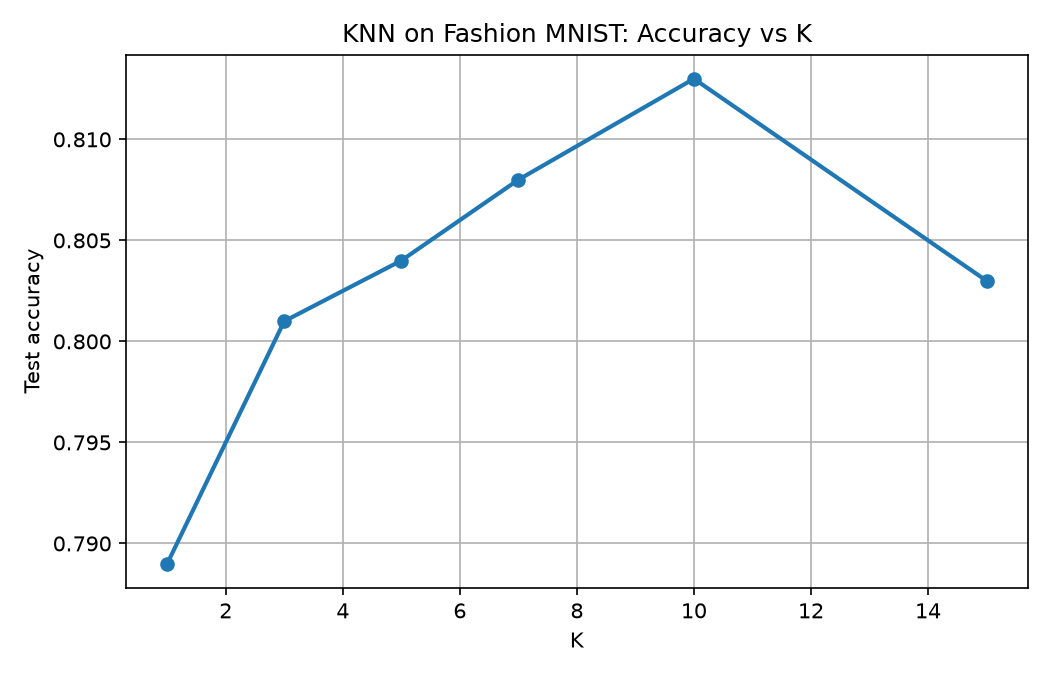
\includegraphics[width=0.78\textwidth]{exp7_acc.png}\par
\small Fig. 1: Test accuracy vs $K$ (peak at $K=10$).\par
\end{center}
\vspace{4pt}

\expheading{RESULT}
\vspace{4pt}
{\fontsize{12}{15}\selectfont
The above program was implemented and executed successfully using Python, and the corresponding output was obtained and verified. The results of the \textbf{K-Nearest Neighbors classification} were analyzed and found to be satisfactory, thereby achieving the desired objective of the experiment.\par
}

\vspace{12pt}

\noindent\textbf{Faculty Signature:} \underline{\hspace{3.6cm}} \hfill \textbf{Date:} \underline{\hspace{2.8cm}}\par

\end{document}
